\chapter{Estado del arte}

\section{Aprendizaje en SNN}

El aprendizaje en SNN se enfrenta a desafíos específicos derivados de la naturaleza binaria y asincrónica de los spikes, así como de la dinámica temporal explícita de las neuronas y sinapsis. \cite{Neftci2019SurrogateGradient, Zenke2021surrogatesnn}. En la literatura se han desarrollado principalmente cinco familias de enfoques: entrenamiento directo mediante gradientes (p. ej. gradientes sustitutos), conversión ANN–SNN, reglas de plasticidad sináptica tipo plasticidad dependiente del tiempo de disparo (Spike-Timing-Dependent Plasticity, STDP), computación de reservorio y métodos de Neuroevolución que optimizan pesos y arquitectura \cite{Bittar2022surrogatespiking, Moisy2006snnsurvey}.

\subsection{Limitaciones del Backpropagation clásico en SNN}
El algoritmo del \textit{Backpropagation} clásico, desarrollado para neuronas con activaciones continuas y derivables, no es directamente aplicable a SNN porque la función de disparo es típicamente una no linealidad tipo función escalón de Heaviside, no derivable y con gradiente nulo casi en todas partes \cite{Zenke2021surrogatesnn}. Adicionalmente, el aprendizaje supervisado en SNN requiere tratar la dimensión temporal de forma explícita, lo que lleva a variantes de Backpropagation Through Time (BPTT) con costes computacionales elevados y problemas de desvanecimiento de gradientes o explosivos sobre horizontes de simulación largos \cite{Neftci2019SurrogateGradient, Bittar2022surrogatespiking}.

En SNN biológicamente plausibles, la dinámica de membrana y de sinapsis introduce estados internos de memoria que complican aún más la asignación de crédito temporal, pues los efectos de un spike presináptico pueden manifestarse tras múltiples pasos de tiempo \cite{Moisy2006snnsurvey}. Por otra parte, la implementación eficiente en hardware neuromórfico exige mantener una actividad de disparo muy dispersa (sparse), lo que agrava los problemas de estimación de gradientes \cite{Li2024snnsparsesurrogate, Schuman2022Opportunities}.

Estas limitaciones han motivado la aparición de métodos alternativos de entrenamiento que aproximan o evitan el cálculo exacto del gradiente, tales como los gradientes sustitutos, la conversión ANN–SNN y los enfoques basados en plasticidad sináptica o en algoritmos evolutivos \cite{Shen2024EvolutionarySNN, Schuman2022Opportunities}.

\subsection{Alternativas al uso de Backpropagation}
A pesar de las limitaciones del Backpropagation en SNN, existen alternativas al entrenamiento de SNN usando algunos métodos y técnicas que se describen a continuación.

\paragraph{Gradientes sustitutos (surrogate gradients)}
Los métodos de gradientes sustitutos aproximan la derivada de la función de disparo no diferenciable mediante una función suave (por ejemplo sigmoide, triangular o cuadrática), lo que permite aplicar variantes de descenso por gradiente y BPTT en SNN de forma análoga a las redes artificiales clásicas \cite{Zenke2021surrogatesnn}. En estos enfoques, durante la fase hacia adelante se mantiene la dinámica de disparo binaria, mientras que en la fase hacia atrás se reemplaza la derivada nula por una aproximación diferenciable en un vecindario del umbral, lo que hace posible propagar señales de error útiles \cite{Neftci2019SurrogateGradient}.

Diversos estudios han mostrado que el aprendizaje con gradientes sustitutos puede alcanzar desempeños competitivos con ANN en tareas de clasificación y reconocimiento de patrones, manteniendo al mismo tiempo ciertas ventajas de eficiencia energética al ejecutarse sobre hardware neuromórfico \cite{Zenke2021surrogatesnn, Schuman2022Opportunities}. Los resultados muestran que el entrenamiento con gradientes sustitutos no depende demasiado de la forma exacta de la función usada como aproximación de la derivada. Sin embargo, sí es importante ajustar adecuadamente su escala y añadir una penalización sobre la actividad de disparo, para evitar redes con demasiados spikes y conservar la esparsidad deseada \cite{Li2024snnsparsesurrogate}.

Trabajos recientes han propuesto extensiones como gradientes sustitutos enmascarados (Masked Surrogate Gradients), que buscan equilibrar la eficacia del entrenamiento con la dispersidad del gradiente, mejorando la capacidad de generalización de las SNN \cite{Li2024snnsparsesurrogate}. Asimismo, se han reportado aplicaciones exitosas de gradientes sustitutos en dominios de procesamiento de voz y comandos de habla, donde SNN entrenadas directamente con este enfoque alcanzan precisiones comparables a arquitecturas ANN convencionales \cite{Bittar2022surrogatespiking}.

\paragraph{Conversión ANN-SNN}
Una alternativa al entrenamiento directo consiste en entrenar primero una red neuronal artificial (ANN) con activaciones continuas (por ejemplo ReLU) y posteriormente convertirla en una SNN manteniendo su topología, trasladando los pesos y ajustando umbrales y codificación temporal \cite{Jiang2023anntosnn, Schuman2022Opportunities}. Esta clase de métodos ha demostrado que es posible obtener SNN profundas con precisiones cercanas a las ANN de origen en conjuntos de datos de gran escala como CIFAR \cite{cifar-10} o ImageNet, aunque el compromiso entre latencia (número de pasos de tiempo) y exactitud sigue siendo un problema central \cite{Ding2021anntosnnoptimal, Gao2023anntosnnbipolarlif}. Para reducir el error de conversión y la latencia, se han propuesto modificaciones en las activaciones de la ANN de origen, como capas específicas de normalización de tasa o funciones ReLU modificadas y cuantizadas que aproximan mejor el comportamiento de neuronas de disparo \cite{Ding2021anntosnnoptimal}.

% También se ha explorado la integración con otras técnicas como entrenamiento consciente de cuantización (quantization-aware training) en el proceso de conversión, evitando fases de postprocesado costosas \cite{Gao2023anntosnnbipolarlif, Jiang2023anntosnn}. Más recientemente, se han introducido esquemas de codificación diferencial que transmiten cambios incrementales de tasa en lugar de tasas absolutas, lo que reduce el número de spikes y el consumo energético sin necesidad de entrenamiento adicional tras la conversión \cite{huang2025differentialanntosnn}.

\paragraph{Plasticidad sináptica (STDP y variantes)}
La plasticidad dependiente del tiempo de disparo (Spike-Timing Dependent Plasticity, STDP) es una regla de aprendizaje inspirada en observaciones neurobiológicas, donde el cambio de peso sináptico depende de la diferencia temporal entre los spikes pre y postsinápticos \cite{RAHMAN2025stdp}. En su forma clásica, los spikes presinápticos que preceden ligeramente a los spikes postsinápticos inducen potenciación de la sinapsis, mientras que spikes postsinápticos anteriores a los presinápticos conducen a depresión, implementando una versión temporizada de aprendizaje Hebbiano \cite{Moisy2006snnsurvey, RAHMAN2025stdp}.

STDP se ha utilizado ampliamente como regla de aprendizaje no supervisado en SNN, permitiendo que las redes aprendan características relevantes de los datos de entrada, y ha sido aplicada sobre hardware emergente como memorias resistivas (RRAM) para aprendizaje en línea \cite{Guo2019rramsnn}. No obstante, algunas variantes de STDP incorporan señales de refuerzo o neuromodulación, lo que permite extender el esquema a escenarios de aprendizaje por refuerzo y supervisado aproximado \cite{RAHMAN2025stdp}.

% Por ejemplo, se han propuesto reglas de STDP moduladas por recompensa (Reward-Modulated STDP, RM‑STDP) que combinan correlaciones temporales locales con señales de recompensa global, logrando resolver tareas no linealmente separables como XOR en configuraciones de computación de reservorio basadas en SNN.

% Además, se han introducido variantes como STDP basada en ensamblajes (assembly-based STDP), que organizan neuronas en conjuntos funcionales y fortalecen selectivamente las conexiones intra-ensamblaje mientras inhiben conexiones inter-ensamblaje para mejorar la capacidad de representación jerárquica.

Aunque STDP y sus extensiones ofrecen una alta plausibilidad biológica y se adaptan bien a implementaciones locales en hardware, presentan desafíos importantes de escalabilidad, sensibilidad a hiperparámetros y dificultad para imponer objetivos globales de tarea en redes profundas \cite{Saranirad2022stdp, RAHMAN2025stdp}.

\paragraph{Computación de reservorio}
El reservorio es una red recurrente de conexiones fijas y generadas aleatoriamente que, al recibir una entrada, actúa como un sistema dinámico no lineal capaz de proyectar la entrada a un espacio de estados de alta dimensión, sin necesidad de entrenamiento alguno \cite{LUKOSEVICIUS2009reservoir}. Teniendo eso en cuenta, la computación de reservorio es un paradigma en el que solo se entrenan los pesos de salida de una red recurrente, manteniendo fijos los pesos internos del reservorio, lo que simplifica el aprendizaje sobre dinámicas no lineales complejas \cite{LUKOSEVICIUS2009reservoir}. Los dos modelos pioneros son las Echo State Networks (ESN), basadas en neuronas de activación continua, y las Liquid State Machines (LSM), que emplean neuronas de espigas y sinapsis dinámicas, representando respectivamente la segunda y la tercera generación de redes neuronales \cite{LUKOSEVICIUS2009reservoir}.

En LSM, el reservorio consiste en una población de neuronas de espigas, donde los patrones de entrada pueden ser linealmente separados por una capa de lectura entrenable \cite{LUKOSEVICIUS2009reservoir}. Estas arquitecturas han demostrado ser capaces de resolver tareas que requieren memoria de corto plazo y no linealidad, como reconocimiento de habla, predicción de series temporales y detección de crisis epilépticas, si bien con un coste computacional mayor que ESN debido a la simulación de spikes \cite{Kholkin2023reservoirsnn}.

En el contexto de SNN, la computación de reservorio presenta la ventaja de evitar el entrenamiento de las conexiones recurrentes internas, delegando el aprendizaje a una capa de salida lineal o ligeramente no lineal que puede optimizarse mediante métodos clásicos de regresión o clasificación \cite{LUKOSEVICIUS2009reservoir}.

% CONSIDERAR PARAGRAPH
\paragraph{Neuroevolución}
La Neuroevolución emplea algoritmos evolutivos para optimizar redes neuronales, tratando pesos, topología y otros hiperparámetros como genotipos que se adaptan mediante operadores de selección, mutación y, en algunos casos, cruce \cite{Hiraga2024mutationbasedevolution}. A diferencia de los métodos basados en gradientes, la Neuroevolución no requiere usar la derivada en la función de coste, lo que la hace especialmente atractiva para problemas con funciones objetivo no diferenciables, ruidosas o definidas por simuladores complejos \cite{risi2025neuroevolution}. El flujo principal de los algoritmos evolutivos se puede ver en la Figura \ref{fig:ea-flujo}.

\begin{figure}
    \centering
    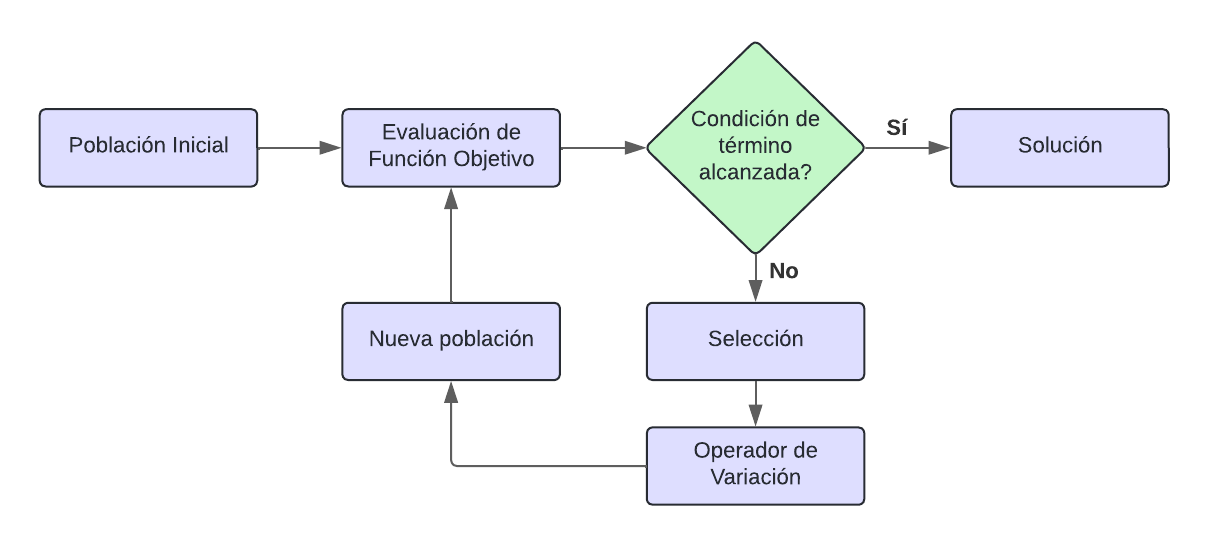
\includegraphics[width=0.8\linewidth]{images/ea-flujo.png}
    \caption{Flujo principal de un algoritmo evolutivo. Se comienza con un conjunto de soluciones candidatas que son evaluadas por una función objetivo. Basado en el desempeño, ciertas soluciones se eligen para producir variabilidad mediante operadores genéticos. El ciclo se repite hasta que se alcanza la condición de término. Adaptado de \cite{risi2025neuroevolution}.}
    \label{fig:ea-flujo}
\end{figure}

En redes neuronales artificiales profundas, se ha demostrado que algoritmos genéticos puros pueden escalar a redes con millones de parámetros, alcanzando rendimientos competitivos con métodos de aprendizaje profundo en tareas de control y refuerzo, lo que evidencia el potencial de la exploración poblacional a gran escala \cite{Stanley2019neuroevolution}. La Neuroevolución también permite optimizar simultáneamente la arquitectura (número de capas, conexiones, tipos de neuronas) y los pesos, abordando de manera unificada problemas de búsqueda de arquitectura neuronal que son difíciles de tratar con \textit{Backpropagation} \cite{Such2017deepneuroevolution, Schuman2022Opportunities}.

Las ventajas principales de la Neuroevolución incluyen: no depender de gradientes ni de funciones objetivo diferenciables, lo que permite optimizar también objetivos no diferenciables o ruidosos; optimizar simultáneamente pesos, arquitectura y otros hiperparámetros; y mantener diversidad poblacional, lo que favorece la exploración y la aparición de soluciones novedosas \cite{Hiraga2024mutationbasedevolution}. Estas características la hacen especialmente atractiva en escenarios donde la dinámica de la red o la función de aptitud se definen mediante simuladores complejos, con recompensas escasas o retardadas, o donde se desean incorporar explícitamente objetivos adicionales como robustez, interpretabilidad o eficiencia energética \cite{risi2025neuroevolution}.

En el ámbito de las SNN, han surgido enfoques evolutivos donde los algoritmos diseñan tanto la topología como los parámetros neuronales (por ejemplo constantes de tiempo y umbrales) y los esquemas de codificación de spikes, logrando redes energéticamente eficientes y de alto rendimiento en diferentes benchmarks \cite{Shen2024EvolutionarySNN}. Estudios recientes han mostrado que la elección del modelo neuronal (por ejemplo Izhikevich frente a LIF) y del esquema de codificación influye de manera crucial en el rendimiento de SNN evolucionadas, lo que resalta la importancia de configurar adecuadamente estos elementos durante la optimización evolutiva \cite{LoyolaJara2026evolvingsnn}.

Las principales ventajas de la Neuroevolución para SNN incluyen su naturaleza libre de gradientes, la capacidad de manejar funciones objetivo no diferenciables (como métricas de energía o esparsidad de spikes) y la posibilidad de optimizar explícitamente pesos, arquitecturas y parámetros neuronales bajo múltiples objetivos \cite{Shen2024EvolutionarySNN, Schuman2022Opportunities}. No obstante, estos métodos presentan desafíos significativos de coste computacional y escalabilidad, ya que requieren evaluar poblaciones completas de redes en cada generación y gestionar espacios de búsqueda de alta dimensión, lo que exige estrategias eficientes de muestreo, paralelización y reducción de complejidad \cite{Hiraga2024mutationbasedevolution, Such2017deepneuroevolution}.

En la literatura reciente se han propuesto marcos unificados que combinan Neuroevolución con aprendizaje por gradiente estocástico, así como algoritmos evolutivos capaces de trabajar con múltiples objetivos como precisión, complejidad del modelo y eficiencia energética, lo que resulta especialmente relevante para el diseño de SNN ejecutables en hardware neuromórfico bajo restricciones de recursos \cite{Zhang2023DNN_Neuroevolution_SGD, Shen2024EvolutionarySNN}. En este contexto, los métodos de optimización evolutiva multiobjetivo aplicados a SNN se alinean de forma natural con la necesidad de equilibrar desempeño, esparsidad y costo computacional en redes de disparo de gran escala, motivando la exploración de algoritmos avanzados de optimización poblacional y estrategias de codificación adecuadas para este tipo de modelos \cite{Shen2024EvolutionarySNN, Hiraga2024mutationbasedevolution}.


%---------------------

\section{Neuroevolución en SNN}
La Neuroevolución se refiere al uso de algoritmos evolutivos para diseñar y entrenar redes neuronales, tratando pesos, arquitectura y otros hiperparámetros como individuos de una población que se adapta mediante selección, mutación y recombinación \cite{Schuman2020evooptineuro, Shen2024EvolutionarySNN}. En el contexto de SNN, esta familia de métodos se ha consolidado como una alternativa a los enfoques basados en gradientes, especialmente cuando se busca optimizar simultáneamente la estructura de la red, los parámetros neuronales y criterios adicionales como eficiencia energética o tamaño del modelo \cite{Shen2024EvolutionarySNN, Schuman2022Opportunities}.

\subsection{Optimización en SNN}
Los trabajos de Neuroevolución aplicados a SNN se diferencian principalmente por el conjunto de elementos que deciden optimizar: pesos sinápticos, topología de la red, parámetros neuronales y esquemas de codificación y decodificación, así como métricas multiobjetivo asociadas al desempeño y la eficiencia estructural \cite{Schliebs2013snn-survey, Jin2007evo-multi-snn}. Los primeros enfoques se centraron en redes relativamente poco profundas, donde algoritmos como GA, PSO, DE y estrategias de armonía se utilizaron para ajustar pesos, retardos sinápticos y conectividad, abordando tareas de clasificación y control con arquitecturas de tamaño moderado \cite{Shen2024EvolutionarySNN}.

En el marco de EONS (Evolutionary Optimization for Neuromorphic Systems) \cite{Schuman2020evooptineuro}, Schuman y colaboradores proponen un esquema evolutivo que optimiza SNN representadas como grafos de nodos y aristas, donde cada nodo y cada sinapsis pueden asociar múltiples parámetros (por ejemplo, umbrales, fugas, pesos y retardos) que se ajustan evolutivamente, permitiendo determinar simultáneamente la estructura de la SNN y los parámetros específicos de cada elemento \cite{Schuman2020evooptineuro}, y se ha aplicado tanto a tareas de clasificación como de control, a problemas de diseño de reservorios y a optimización multiobjetivo orientada a minimizar el tamaño de la red \cite{Schuman2022Opportunities}.

Otros trabajos utilizan Neuroevolución principalmente para búsqueda de arquitecturas para posterior entrenamiento usando Backpropagation, integrando mecanismos como Neural Architecture Search (NAS) en el dominio de las SNN; por ejemplo, los enfoques AutoSNN, SpikeDHS, NeuEvo y STTS emplean algoritmos evolutivos o híbridos para escoger bloques de convolución, tamaños de kernel, conexiones recurrentes y tipos de operadores de disparo, con énfasis en el compromiso entre precisión, tasa de espigas y coste computacional \cite{Shen2024EvolutionarySNN}, y se han reportado arquitecturas que alcanzan precisiones competitivas en CIFAR, ImageNet y tareas sobre datos de eventos, manteniendo un número de operaciones sinápticas significativamente menor que redes artificiales equivalentes \cite{Shen2024EvolutionarySNN}.

También existe una línea de trabajo centrada en la optimización directa de la arquitectura y los hiperparámetros de SNN mediante marcos de Neuroevolución generalistas, como SPENSER \cite{Branquinho2023-neuro-conv-snn}, que extiende un framework evolutivo originalmente diseñado para ANN (DENSER) al caso de SNN convolucionales, generando redes con rendimiento competitivo en tareas de clasificación estática.

Finalmente, una línea particularmente relevante para esta tesis considera la optimización multiobjetivo de SNN, donde algoritmos evolutivos buscan simultáneamente minimizar el error de clasificación y reducir el tamaño o la complejidad de la red, dando lugar a frentes de Pareto que exponen el compromiso entre exactitud y esparsidad \cite{Schuman2022Opportunities, Jin2007evo-multi-snn}. En estos trabajos, los objetivos incluyen típicamente métricas de desempeño (exactitud, error) y medidas estructurales como número de neuronas activas, porcentaje de conexiones no nulas o estimaciones de consumo energético asociadas al número de operaciones sinápticas, lo que se alinea de forma directa con el enfoque de optimización esparsa considerado en este trabajo de título \cite{dimovska2020multiobjectiveoptimizationsizeresilience}.


\subsection{Ventajas del enfoque evolutivo en SNN}
Una de las ventajas más citadas de la Neuroevolución en el contexto de SNN es que los algoritmos evolutivos no requieren información de gradiente, por lo que pueden trabajar directamente con funciones de activación no diferenciables, dinámicas temporales complejas y simuladores neuromórficos que no ofrecen derivadas de la función de coste \cite{Schuman2022Opportunities, Schuman2020evooptineuro}. Esta independencia de gradientes permite aplicar los métodos evolutivos a arquitecturas recurrentes, redes con retardos axonales y sinápticos, y modelos neuronales biológicamente plausibles (como Izhikevich \cite{Izhikevich2003} o LIF \cite{Gao2023anntosnnbipolarlif}) sin modificar sus ecuaciones subyacentes, lo que constituye una ventaja frente a los enfoques basados en gradientes sustitutos \cite{Shen2024EvolutionarySNN}.

Otra ventaja relevante es la capacidad de optimizar simultáneamente la estructura y los parámetros de la red, abarcando desde el número de neuronas y capas hasta el patrón de conectividad y los valores de umbral, pesos y retardos, tal como se ejemplifica en EONS y en marcos inspirados en NEAT \cite{Schuman2020evooptineuro, Stanley2002NEAT}. Este tratamiento unificado del diseño de arquitectura y del ajuste de parámetros permite explorar configuraciones que serían difíciles de alcanzar mediante procedimientos clásicos haciendo uso de gradientes, y facilita la aparición de topologías no convencionales que utilizan ciclos, conexiones cruzadas e interacciones complejas entre capas \cite{Elbrecht2020-neuro-snn, Schuman2020evooptineuro}.

Los algoritmos evolutivos también se adaptan de forma natural a escenarios multiobjetivo, incorporando explícitamente objetivos como exactitud, tamaño de la red, consumo energético o robustez frente a perturbaciones, y utilizando indicadores como Hipervolumen o IGD para evaluar la calidad del conjunto de soluciones encontradas \cite{Jin2007evo-multi-snn, dimovska2020multiobjectiveoptimizationsizeresilience}. En el contexto neuromórfico, esta capacidad resulta especialmente útil cuando se desea reducir el número de conexiones activas, limitar el rango de pesos o respetar restricciones de resolución y retardos impuestos por el hardware, sin perder de vista el rendimiento en la tarea de clasificación o control \cite{Branquinho2023-neuro-conv-snn, Schuman2020evooptineuro, Schuman2022Opportunities}.

Otro aspecto ventajoso es la compatibilidad de los métodos evolutivos con tareas de control y refuerzo, donde la función objetivo puede ser no diferenciable, ruidosa o definida por simuladores complejos; diversos trabajos han mostrado que estrategias evolutivas pueden entrenar SNN para problemas como navegación de robots y juegos, alcanzando comportamientos comparables o superiores a reglas de plasticidad locales como STDP-RL \cite{Hasegan2022snn-rl, Shen2024EvolutionarySNN}.

Finalmente, los enfoques evolutivos ofrecen una integración relativamente directa con plataformas neuromórficas reales, ya que pueden incluir en la representación genética los límites de hardware (por ejemplo, resolución de pesos, número máximo de retardos, topologías permitidas) y evolucionar únicamente redes que sean realizables bajo dichas restricciones.

%--------

\subsection{Limitaciones actuales y desafíos}
A pesar de sus ventajas, los métodos evolutivos aplicados a SNN presentan limitaciones importantes en términos de coste computacional, ya que requieren evaluar poblaciones completas de redes en cada generación, y cada evaluación implica simulaciones temporales potencialmente largas sobre conjuntos de datos de entrenamiento \cite{Schuman2022Opportunities, Schuman2020evooptineuro}. Esta naturaleza poblacional hace que la Neuroevolución sea, en muchos casos, más lenta para converger que los enfoques basados en gradientes, especialmente cuando se trabaja con redes profundas y datasets de gran escala, lo que ha motivado el desarrollo de estrategias de reducción de coste y búsqueda más eficiente \cite{Shen2024EvolutionarySNN, Branquinho2023-neuro-conv-snn}.

Históricamente, muchas aplicaciones evolutivas en SNN se han limitado a arquitecturas relativamente poco profundas o a problemas con pocas entradas, debido tanto a restricciones de hardware como a la complejidad de simular grandes SNN; aunque trabajos recientes han extendido estos métodos a SNN profundas y convolucionales, todavía existe una brecha respecto del rendimiento y la escala alcanzados por redes artificiales entrenadas con gradientes sustitutos o conversión ANN-SNN \cite{Branquinho2023-neuro-conv-snn, Schliebs2013snn-survey}. Algunos estudios \cite{Shen2024EvolutionarySNN} señalan que aunque enfoques como SpikeDHS, STTS, AutoSNN y NeuEvo logran precisiones competitivas en CIFAR e ImageNet, muchos de ellos dependen de espacios de búsqueda complejos, entrenamiento de superredes o combinaciones con técnicas basadas en gradientes, lo que evidencia que la Neuroevolución pura aún enfrenta desafíos en tareas de muy gran escala.

Otro desafío importante reside en el diseño del espacio de búsqueda y la codificación genética de las redes, ya que la elección de cómo representar arquitectura, pesos, retardos y operadores de disparo influye de manera crítica en la capacidad del algoritmo evolutivo para explorar soluciones útiles sin perder eficiencia \cite{Elbrecht2020-neuro-snn}. Además, existe aún poca homogeneidad en la literatura respecto de los criterios de evaluación y los benchmarks utilizados para comparar métodos evolutivos en SNN, lo que dificulta construir una imagen clara de cuál enfoque ofrece el mejor compromiso entre precisión, esparsidad y coste computacional \cite{Shen2024EvolutionarySNN}. Algunos trabajos reportan únicamente métricas de exactitud, mientras que otros añaden medidas de tasa de espigas, número de sinapsis activas o estimaciones de consumo energético. La falta de conjuntos de pruebas estandarizados para SNN evolutivas hace que los resultados sean, en muchos casos, difíciles de trasladar entre dominios y plataformas de hardware \cite{dimovska2020multiobjectiveoptimizationsizeresilience, Shen2024EvolutionarySNN}.

Finalmente, aunque las aproximaciones evolutivas han mostrado resultados prometedores en aplicaciones de control y clasificación, su combinación con requisitos estrictos de esparsidad y gran escala sigue siendo un problema abierto, donde la búsqueda de arquitecturas extremadamente ligeras y redes altamente eficientes debe equilibrarse con la necesidad de mantener un rendimiento comparable al de enfoques basados en gradientes \cite{dimovska2020multiobjectiveoptimizationsizeresilience, Schuman2020evooptineuro}. Esta tensión entre exploración evolutiva, exigencias de hardware neuromórfico y objetivos multiobjetivo complejos motiva el desarrollo de algoritmos evolutivos especializados para problemas esparsos de gran escala, como los SMOEA considerados en esta tesis, que buscan mejorar la capacidad de las SNN evolutivas para operar en escenarios donde la eficiencia estructural es tan relevante como la precisión \cite{Shen2024EvolutionarySNN, Schuman2022Opportunities}.

%------------

\section{Esparsidad y eficiencia estructural de redes neuronales}

\subsection{Definición}
En el contexto de redes neuronales profundas y SNN, se entiende por modelo esparso aquel en que una fracción significativa de los parámetros o conexiones toma el valor cero, de modo que solo un subconjunto reducido de sinapsis participa efectivamente en el cómputo \cite{REINERS2022sparse, Huang2021sparse-opti-multi}. Esta reducción explícita de conexiones activas se traduce en una menor complejidad estructural del modelo, con impacto directo sobre el número de operaciones requeridas, el uso de memoria y, en plataformas neuromórficas, el consumo energético asociado a eventos sinápticos \cite{LIAN2024-multi-cnn-ea, Schuman2022Opportunities, REINERS2022sparse}.

Diversos trabajos sobre poda y compresión de redes neuronales formulan la búsqueda de arquitecturas esparsas como un problema de optimización multiobjetivo, donde se busca simultáneamente preservar el desempeño predictivo y disminuir la complejidad estructural del modelo \cite{Huang2021sparse-opti-multi, REINERS2022sparse}. En el caso particular de SNN, estudios recientes \cite{dimovska2020multiobjectiveoptimizationsizeresilience, Schuman2022Opportunities} han mostrado que minimizar de forma explícita el tamaño o número de conexiones de la red puede incrementar la resiliencia a fallos hardware y reducir el coste de implementación en arquitecturas neuromórficas, manteniendo una precisión de clasificación aceptable.

Así, la esparsidad pasa a constituir un objetivo explícito de diseño, que debe equilibrarse con la exactitud y otras métricas de rendimiento mediante por ejemplo, técnicas de optimización basada en poblaciones como los algoritmos evolutivos \cite{REINERS2022sparse, Huang2021sparse-opti-multi}. Este enfoque resulta coherente con la motivación neuromórfica de la tesis, donde el entrenamiento de SNN busca no solo resolver correctamente tareas de clasificación, sino hacerlo con redes estructuralmente ligeras y eficientes en términos de recursos computacionales \cite{dimovska2020multiobjectiveoptimizationsizeresilience, Schuman2022Opportunities}.

En la literatura de poda de redes densas se distingue entre esparsidad no estructurada y esparsidad estructurada \cite{Yang2019-mo-cnn-ga, LIAN2024-multi-cnn-ea}. Los métodos de poda no estructurada generan patrones irregulares de pesos nulos que pueden ser difíciles de explotar en hardware convencional, ya que las bibliotecas estándar de convolución no suelen estar optimizadas para kernels extremadamente dispersos sin soporte especializado \cite{HIRSCH2022-mo-dnn-drl, LIAN2024-multi-cnn-ea}. 

En cambio, la esparsidad estructurada tiende a traducirse en reducciones más evidentes del coste computacional, ya que elimina operaciones completas asociadas a filtros o canales y permite reutilizar implementaciones de convolución estándar con menores dimensiones efectivas \cite{Chen2021-sparse-nn-moo, LIAN2024-multi-cnn-ea, HIRSCH2022-mo-dnn-drl}. Sin embargo, incluso en redes densas de activaciones continuas, diversos trabajos han mostrado que la elección del tipo de esparsidad y la granularidad de la poda influyen en el compromiso alcanzado entre precisión, tamaño del modelo y latencia de inferencia \cite{REINERS2022sparse, Yang2019-mo-cnn-ga}.

En SNN, la noción de esparsidad se puede extender desde la estructura de pesos hacia la actividad temporal, considerando tanto el número de sinapsis activas como la tasa de espigas generada por la red durante la inferencia \cite{dimovska2020multiobjectiveoptimizationsizeresilience, Jin2007evo-multi-snn, Schuman2022Opportunities}. Por ello, la tesis adopta una noción de esparsidad estructural basada en el número de conexiones activas, alineada con trabajos que consideran explícitamente el tamaño de la red o la fracción de pesos no nulos como objetivos a minimizar, además de la precisión de clasificación \cite{Huang2021sparse-opti-multi, dimovska2020multiobjectiveoptimizationsizeresilience}. Esta formulación permite vincular de forma directa la optimización evolutiva de SNN con el objetivo de obtener redes más compactas y eficientes, coherentes con los requisitos de ejecución en hardware neuromórfico \cite{LIAN2024-multi-cnn-ea, Schuman2022Opportunities}.

Un resultado recurrente en la literatura es que la reducción del número de parámetros o conexiones de una red mejora su eficiencia pero, más allá de cierto umbral, tiende a degradar significativamente la exactitud, lo que evidencia un compromiso intrínseco entre rendimiento y esparsidad \cite{REINERS2022sparse}. Estudios sobre poda multiobjetivo \cite{LIAN2024-multi-cnn-ea, HIRSCH2022-mo-dnn-drl} de redes densas muestran que tratar la exactitud y la complejidad estructural como objetivos separados permite obtener frentes de Pareto que contienen tanto modelos muy precisos y relativamente densos como modelos altamente comprimidos con una degradación moderada del desempeño.

Trabajos recientes sobre entrenamiento y compresión esparsa señalan que formular el problema como optimización multiobjetivo permite descubrir automáticamente niveles de esparsidad adecuados para cada arquitectura y conjunto de datos \cite{chen2026multiobjective-llm, Huang2021sparse-opti-multi, Huang2021sparse-opti-multi}. En este contexto, algoritmos evolutivos jerárquicos y esquemas de búsqueda multiobjetivo han demostrado que es posible reducir hasta la mitad del número de parámetros de redes convolucionales manteniendo prácticamente la misma precisión, lo que ilustra la utilidad de estrategias de exploración poblacional \cite{khan2026hierarchicalimportanceguidedmultiobjectiveevolutionary, Yang2019-mo-cnn-ga}. Este planteamiento permite comparar directamente modelos evolutivos de SNN con redes equivalentes basadas en ANN, identificando en qué regiones del frente de Pareto el enfoque de optimización esparsa multiobjetivo resulta más ventajoso en términos de eficiencia estructural.


\subsection{Métricas para evaluar esparsidad y eficiencia estructural}
Las aplicaciones de poda y compresión esparsa utilizan de forma habitual métricas de desempeño como la exactitud o el error de clasificación sobre conjuntos de prueba, que capturan la capacidad predictiva del modelo después de aplicar las transformaciones de esparsidad \cite{REINERS2022sparse, Huang2021sparse-opti-multi}. A la vez, incorporan indicadores de complejidad estructural, como el número total de parámetros y el porcentaje de pesos no nulos \cite{Chen2021-sparse-nn-moo, LIAN2024-multi-cnn-ea}.

Estudios recientes sobre SNN evolutivas \cite{Shen2024EvolutionarySNN} reportan explícitamente el número de espigas, operaciones sinápticas y consumo teórico de energía junto con la precisión en benchmarks como CIFAR e ImageNet, mostrando que arquitecturas obtenidas mediante métodos evolutivos pueden alcanzar reducciones significativas de operaciones sinápticas con exactitud comparable a redes densas \cite{Branquinho2023-neuro-conv-snn, LIAN2024-multi-cnn-ea}.

Cuando la optimización se plantea como un problema multiobjetivo, la calidad del conjunto de soluciones se evalúa frecuentemente mediante indicadores globales como el Hipervolumen, que mide el volumen de la región del espacio de objetivos dominada por el frente aproximado respecto de un punto de referencia \cite{Jin2007evo-multi-snn, dimovska2020multiobjectiveoptimizationsizeresilience}, permitiendo integrar en una sola cifra información de convergencia hacia el frente de Pareto verdadero y de diversidad a lo largo del frente, resultando adecuado para comparar diferentes algoritmos evolutivos en términos de su capacidad para generar soluciones que equilibren exactitud y esparsidad \cite{Zitzler2007HV_revisited}. Otros indicadores, como la Distancia Generacional Invertida (IGD), se han utilizado para cuantificar la proximidad del frente aproximado a un conjunto de referencia, lo que es útil cuando se dispone de soluciones conocidas o se desea evaluar la consistencia del comportamiento del algoritmo en distintos problemas \cite{dimovska2020multiobjectiveoptimizationsizeresilience}. En trabajos sobre compresión esparsa de redes densas, estos indicadores se combinan con métricas de tamaño de modelo y coste de cómputo para caracterizar de forma más completa la calidad del conjunto de configuraciones obtenidas.

%-------------

\section{Optimización esparsa multiobjetivo a gran escala}
Los problemas de optimización multiobjetivo cuyas soluciones óptimas son esparsas y que involucran un gran número de variables de decisión se conocen en la literatura como \textit{sparse multi-objective optimization problems} (SMOPs) \cite{Shao2025_SMOEA, Tian2020AnEALSMOP}. En estos problemas, la mayoría de las variables toman valor cero en las soluciones óptimas, pero el número total de variables puede ser del orden de cientos o miles, lo que genera un espacio de búsqueda extremadamente grande y difícil de explorar con presupuestos de evaluación limitados \cite{Tian2020AnEALSMOP, ZOU2025-sparse-LSMOEA, Shao2025_SMOEA}.

Este tipo de problemas aparece en dominios como reconstrucción de señales, detección de nodos críticos en grafos, ataques adversarios y modelos neuronales esparsos \cite{Shao2026AnEA-LSMOP, ZOU2025-sparse-LSMOEA, Shao2025_SMOEA}, donde se desea identificar pocos parámetros relevantes sin perder desempeño en múltiples objetivos en conflicto. En el contexto de redes neuronales, la formulación multiobjetivo con términos de error y esparsidad permite tratar explícitamente el compromiso entre precisión de clasificación y complejidad estructural del modelo, alineando la optimización con requisitos de eficiencia computacional y energética \cite{Hotegni2024moo-sparse, REINERS2022sparse}.

Los algoritmos evolutivos multiobjetivo generales (MOEA) han demostrado ser eficaces en problemas con pocos objetivos y dimensiones moderadas, pero su rendimiento se degrada cuando deben encontrar soluciones esparsas en espacios de muy alta dimensión \cite{Hua2021MOEA, Shao2025_SMOEA}. Para abordar esta combinación de gran escala y esparsidad, la comunidad ha desarrollado algoritmos evolutivos multiobjetivo esparsos (SMOEA) que incorporan mecanismos específicos para identificar y mantener variables no nulas, explotando de forma más eficiente la estructura esparsa de las soluciones óptimas \cite{Tian2020AnEALSMOP, HUANG2025-enhanced-moea-lsmo}.

En el escenario de entrenamiento de SNN, estos algoritmos ofrecen un marco natural para optimizar simultáneamente el rendimiento de clasificación y el número de conexiones activas, lo que resulta especialmente relevante cuando se pretende implementar las redes en hardware neuromórfico con restricciones de recursos \cite{REINERS2022sparse, dimovska2020multiobjectiveoptimizationsizeresilience}. El presente trabajo de título se apoya precisamente en esta línea, utilizando SMOEA diseñados para problemas esparsos de gran escala como núcleo del proceso de entrenamiento evolutivo de SNN con objetivos explícitos de precisión y esparsidad estructural \cite{Shao2025_SMOEA}.


\subsection{De MOEA a SMOEA}
Los MOEA clásicos fueron concebidos para problemas donde todas las variables de decisión son potencialmente relevantes y las soluciones de Pareto no presentan estructuras de esparsidad pronunciadas, por lo que aplican operadores de variación y selección de forma prácticamente uniforme sobre todas las dimensiones \cite{TIAN2024-lsmoea, Hua2021MOEA}. En problemas esparsos de gran escala, esta estrategia lleva a dedicar la mayor parte del presupuesto de evaluaciones a modificar variables que deberían permanecer en cero, lo que reduce la eficiencia de la búsqueda y dificulta identificar el subconjunto crítico de variables no nulas \cite{Shao2025_SMOEA}.

Diversos estudios comparativos muestran que MOEA diseñados para grandes dimensiones, pero sin mecanismos específicos de detección de esparsidad tienden a converger hacia soluciones densas que no cumplen los requisitos de número de variables activas, aun cuando ofrecen buen rendimiento en exactitud \cite{ZOU2025-sparse-LSMOEA, Wang2025-ea-genetic-large-scale}. La coexistencia de alta dimensionalidad y esparsidad exacerba el conflicto entre exploración y explotación, ya que el algoritmo debe descubrir simultáneamente qué variables deben activarse y qué valores deben tomar, todo ello en un espacio de búsqueda dominado por configuraciones subóptimas densas \cite{Tian2020AnEALSMOP, Shao2026AnEA-LSMOP}.

Para superar estas limitaciones, los SMOEA introducen operadores genéticos que separan explícitamente la identificación de variables no nulas de la optimización de sus valores, de forma que la presión selectiva pueda concentrarse en la estructura esparsa \cite{HUANG2025-enhanced-moea-lsmo, SparseEA2}. Este cambio de paradigma permite que el algoritmo dedique más evaluaciones a refinar la parte real de las variables activas, manteniendo al mismo tiempo la esparsidad global de las soluciones y mejorando la calidad del frente de Pareto obtenido \cite{SparseEA2, ZOU2025-sparse-LSMOEA}.


\subsection{Familias de SMOEA}
Un estudio reciente \cite{Shao2025_SMOEA} clasifica los SMOEA en tres familias: \textit{métodos basados en nuevos operadores de variación}, \textit{reducción de dimensionalidad} y \textit{agrupamiento de variables de decisión}. La base representacional predominante detrás de esta taxonomía es la codificación bi-nivel, introducida por SparseEA, que representa una solución mediante dos componentes: un vector binario que determina qué variables permanecen activas y un vector real que define sus valores. Esta separación es importante porque permite optimizar simultáneamente la estructura de la solución, identificando las variables relevantes y sus parámetros, controlando explícitamente la esparsidad durante el proceso evolutivo \cite{Tian2020AnEALSMOP, HUANG2025-enhanced-moea-lsmo}. Sin embargo, esta codificación no es universal: como se detalla en la siguiente subsección, algunos algoritmos basados en nuevos operadores de variación prescinden deliberadamente de ella. El detalle de la taxonomía se puede ver en la Tabla \ref{tab:taxonomia-smoea} del Anexo.

Más allá de esta representación, las tres familias se diferencian principalmente en el mecanismo que emplean para identificar y explotar las variables relevantes. La primera familia diseña operadores de variación que favorecen la activación y optimización de variables relevantes; la segunda proyecta la búsqueda hacia subespacios de menor dimensionalidad para reducir el costo computacional; y la tercera agrupa variables relacionadas para optimizarlas por subcomponentes \cite{Shao2025_SMOEA, TIAN2024-lsmoea}. Aunque emplean mecanismos distintos, las tres familias buscan distinguir las variables críticas de aquellas prescindibles y concentrar el esfuerzo evolutivo en las primeras. Por ello, los SMOEA son particularmente adecuados para entrenar SNN, donde es necesario equilibrar la calidad funcional de la red con la reducción de conexiones activas.


\subsection{Algoritmos relevantes}\label{subsec:algoritmos_relevantes}
Dentro de la familia de SMOEA basados en operadores de variación, S-NSGA-II se propone como una extensión de NSGA-II que incorpora operadores genéticos específicos para problemas esparsos de gran escala, mejorando la capacidad de detectar y mantener patrones de esparsidad en las soluciones óptimas \cite{10066873_S-NSGA-II, Shao2025_SMOEA}. A diferencia de los enfoques bi-nivel, S-NSGA-II no introduce una representación adicional para codificar la esparsidad: cada individuo se representa mediante un único vector real de decisión

\begin{equation}
x = (x_1, x_2, \ldots, x_D), \qquad x_j \in [l_j, u_j] \subset \mathbb{R}, \qquad j = 1,\ldots,D,
\end{equation}

donde $x_j = 0$ indica que la $j$-ésima variable permanece inactiva y $x_j \neq 0$ indica que está activa con ese valor, de modo que el patrón de esparsidad es una propiedad emergente del propio vector y no un componente separado del genotipo. Sobre esta codificación de una sola capa actúan sus operadores de cruce y mutación, Sparse Simulated Binary Crossover (S-SBX) y Sparse Polynomial Mutation (S-PM), que distinguen explícitamente entre posiciones activas e inactivas para decidir, en cada cruce o mutación, si una posición conserva su valor, se reactiva o se anula, preservando así la estructura esparsa de los padres mientras exploran regiones relevantes del espacio de objetivos \cite{10066873_S-NSGA-II}.

Los estudios experimentales reportados en la literatura muestran que S-NSGA-II alcanza resultados competitivos frente a otros SMOEA en conjuntos de problemas esparsos multiobjetivo (SMOP), produciendo frentes con buen hipervolumen y diversidad bajo presupuestos de evaluación limitados, evitando además el costo adicional de sincronizar una representación bi-nivel \cite{10066873_S-NSGA-II}. Su diseño mantiene la de dominancia de Pareto y diversidad de NSGA-II, pero adaptada a contextos donde la mayoría de las variables óptimas deben permanecer en cero, lo que lo convierte en un candidato adecuado para problemas de optimización de redes esparsas.

Por otro lado, \textit{Multiobjective Evolutionary Algorithm with Cross-Scale Knowledge Fusion} (MOEA-CKF) \cite{MOEA/CKF} representa una línea de trabajo que sí adopta una codificación bi-nivel explícita. Cada solución se representa mediante el par $(m, d)$, donde $m \in \{0,1\}^D$ es un vector binario que determina qué variables permanecen activas y $d \in \mathbb{R}^D$ es un vector real que almacena sus valores, de forma que el vector de decisión efectivamente evaluado se obtiene componente a componente como

\begin{equation}
x_j = m_j \cdot d_j, \qquad j = 1,\ldots,D.
\end{equation}

Esta separación permite que $d$ se siga optimizando incluso en posiciones actualmente inactivas ($m_j = 0$), conservando información que puede reactivarse en generaciones posteriores, algo que la codificación de una sola capa de S-NSGA-II no contempla. Sobre esta base, MOEA-CKF emplea estrategias de agrupamiento de variables y modelos auxiliares para guiar la búsqueda hacia subespacios donde las variables no nulas pueden optimizarse más intensamente, al tiempo que se mantiene el control sobre la esparsidad global del conjunto de soluciones mediante $m$.

Los resultados reportados para MOEA-CKF en benchmarks de \textit{optimización esparsa multiobjetivo a gran escala} indican mejoras significativas frente a SparseEA y otros SMOEA en términos de convergencia y calidad de la relación entre esparsidad y desempeño. En particular, la capacidad de este algoritmo para aprovechar información aprendida sobre correlaciones entre variables permite dedicar más evaluaciones a refinar los valores de las variables activas, lo que es crucial cuando el número de evaluaciones disponibles es limitado.

% Aunque ambos algoritmos pueden abordar los mismos tipos de problemas, difieren fundamentalmente en la codificación de la esparsidad: S-NSGA-II la representa de forma implícita mediante los ceros de un único vector real, mientras que MOEA-CKF la representa de forma explícita mediante una máscara binaria separada del vector de valores. 

Para una revisión detallada, en el Anexo \ref{chap:anexo-pseudo} se encuentran los pseudocódigos de los algoritmos internos utilizados por MOEA-CKF y S-NSGA-II.

% \textbf{REVISAR}
% En este trabajo se consideran S-NSGA-II y MOEA-CKF como algoritmos evolutivos centrales, dado que ambos han sido diseñados específicamente para SMOPs de gran escala y han demostrado buen rendimiento en la generación de frentes de Pareto esparsos bajo recursos computacionales acotados. Su combinación con modelos de SNN permite estudiar de manera sistemática cómo los mecanismos de optimización esparsa multiobjetivo a gran escala afectan al entrenamiento de SNN, tanto en términos de precisión como de eficiencia estructural y potencial de resiliencia.
% \textbf{REVISAR}

\subsection{Operadores genéticos en SMOEA}\label{subsec:operadores_geneticos}
Los MOEA clásicos, como NSGA-II, se basan en un ciclo compuesto por la inicialización de una población, operadores de variación como cruce y mutación, y selección ambiental. El cruce combina información de soluciones progenitoras, la mutación introduce modificaciones para explorar nuevas regiones del espacio de búsqueda y la selección conserva las soluciones no dominadas que mantienen un buen equilibrio entre convergencia hacia el frente de Pareto y diversidad \cite{Deb2002NSGAII}.

Los SMOEA adaptan este esquema para optimizar no solo los valores de las variables, sino también cuáles de ellas deben permanecer activas. Por ejemplo, S-NSGA-II incorpora una inicialización que cubre distintos patrones de esparsidad, junto con operadores de cruce y mutación que preservan o modifican controladamente tanto los valores de las variables como su estado activo o inactivo. Así, el algoritmo evita generar soluciones innecesariamente densas y puede explorar configuraciones con diferentes niveles de esparsidad.

MOEA-CKF emplea una codificación bi-nivel, formada por una capa binaria que representa el patrón de activación y una capa real que almacena los valores de las variables. Sus operadores utilizan información obtenida durante la evolución para identificar variables relevantes, reducir la dimensión efectiva del problema y agrupar variables con comportamiento relacionado. Luego, aplican variación guiada dentro de estos subconjuntos, utilizando el patrón binario para orientar la optimización de los valores reales. De esta forma, MOEA-CKF integra la búsqueda de una estructura esparsa con el ajuste de los parámetros continuos, concentrando el esfuerzo computacional en las variables más relevantes.


%------------------------


% \subsection{Algoritmos evolutivos multiobjetivo (MOEA)}
% Los algoritmos evolutivos multiobjetivo (MOEA, por sus siglas en inglés) son una familia de métodos metaheurísticos que emplean poblaciones de soluciones y operadores inspirados en la evolución biológica para aproximar conjuntos de soluciones de Pareto en problemas con objetivos en conflicto \cite{Hua2021MOEA}. A diferencia de los métodos clásicos basados en programación matemática, que suelen buscar una única solución óptima agregando los objetivos mediante ponderaciones o funciones escalarizadas, los MOEA mantienen explícitamente un conjunto de individuos y explotan la noción de dominancia de Pareto para construir una aproximación al frente completo en una única corrida del algoritmo \cite{Hong2024LSMOP, Deb2001MOEA}.

% En un MOEA típico, cada individuo codifica una solución candidata $x\in \Omega$ y la población evoluciona mediante selección, recombinación y mutación, de manera que las soluciones no dominadas y bien distribuidas en el espacio de objetivos tienen mayor probabilidad de sobrevivir y generar descendencia \cite{risi2025neuroevolution, Hiraga2024mutationbasedevolution}. El criterio de selección suele combinar un mecanismo de orden parcial basado en la dominancia de Pareto con medidas de diversidad, como la distancia de crowding o indicadores de densidad, con el fin de equilibrar convergencia hacia el frente verdadero y diversidad a lo largo del mismo \cite{Tian2022EAforLSMOP, risi2025neuroevolution}.

% Los MOEA se han consolidado como una herramienta estándar para problemas de ingeniería y ciencias aplicadas, ya que permiten obtener en una sola ejecución un conjunto de soluciones de compromiso que representan diferentes puntos del frente de Pareto y que pueden ser posteriormente evaluadas por el decisor según preferencias adicionales \cite{Hua2021MOEA, Hong2024LSMOP}. Entre los algoritmos representativos se encuentran NSGA-II, SPEA2 y sus extensiones, los cuales emplean ordenamiento rápido por frentes no dominados, elitismo y operadores de diversidad para alcanzar frentes bien aproximados en términos de hipervolumen, distancia generacional invertida (IGD, por sus siglas en inglés) y otras métricas \cite{Hong2024LSMOP, Deb2001MOEA}.

% Desde una perspectiva algorítmica, los MOEA pueden clasificarse según el mecanismo principal de selección en enfoques basados en dominancia de Pareto, en descomposición del problema multiobjetivo en subproblemas escalarizados y en indicadores de calidad, cada uno con ventajas específicas frente a distintos tipos de frentes y estructuras del espacio de búsqueda \cite{Deb2001MOEA}. En particular, los métodos basados en dominancia son robustos y conceptualmente simples, los métodos por descomposición pueden manejar con mayor eficacia un número elevado de objetivos, y los enfoques guiados por indicadores permiten incorporar directamente métricas de desempeño como el hipervolumen en el proceso de selección \cite{Tian2022EAforLSMOP}.

% En el contexto de redes neuronales, los MOEA se han utilizado para optimizar simultáneamente la exactitud de clasificación y la complejidad del modelo, aprovechando la capacidad de los algoritmos evolutivos para explorar espacios de búsqueda no diferenciables, multimodales y de alta dimensión donde los métodos basados en gradientes presentan limitaciones \cite{Tian2022EAforLSMOP, Schuman2022Opportunities}.



% \subsection{Algoritmos evolutivos multiobjetivo esparsos (SMOEA)}
% Los algoritmos evolutivos multiobjetivo esparsos, o \textit{sparse multi-objective evolutionary algorithms} (SMOEA), constituyen una familia de métodos diseñados específicamente para resolver problemas multiobjetivo cuyas soluciones de Pareto son esparsas, es decir, problemas en los que la mayoría de las variables de decisión de las soluciones óptimas toman el valor cero \cite{Shao2025_SMOEA, Hong2024LSMOP}. Este tipo de problemas, denominados sparse multi-objective optimization problems (SMOPs), aparece con frecuencia en dominios científicos e ingenieriles donde coexisten múltiples objetivos en conflicto, un gran número de variables de decisión y una estructura subyacente de esparsidad en las soluciones deseadas \cite{Shao2025_SMOEA}. Debido a esa combinación de alta dimensionalidad y esparsidad, la búsqueda de soluciones de Pareto en SMOPs resulta especialmente difícil bajo recursos computacionales limitados \cite{Shao2025_SMOEA}.

% Aunque los MOEA convencionales han mostrado buen desempeño en numerosos problemas multiobjetivo, su rendimiento tiende a deteriorarse cuando se aplican directamente a SMOPs. El estudio de SMOEAs \cite{Shao2025_SMOEA} señala que incluso muchos MOEA diseñados para problemas multiobjetivo a gran escala presentan dificultades en este contexto, ya sea porque requieren demasiadas evaluaciones para identificar relaciones complejas entre variables o porque pierden direcciones de búsqueda útiles al reducir el espacio de decisión de forma agresiva. En consecuencia, los SMOEA surgen como una especialización de los MOEA tradicionales, incorporando mecanismos explícitos para identificar variables no nulas y explotar la estructura esparsa del frente de Pareto.

% Un elemento central en esta línea de investigación es el esquema de codificación bi-nivel introducido por SparseEA \cite{SparseEA2}, en el cual cada solución se representa mediante un vector binario y un vector real. En este esquema, el vector binario determina qué posiciones de la solución son cero o no cero, mientras que el vector real especifica el valor de las variables activas, de modo que la solución final resulta de la combinación de ambas capas. Según el estudio, esta estrategia se convirtió en una base metodológica ampliamente adoptada por numerosos SMOEA posteriores, debido a que separa de manera natural la búsqueda de la estructura de esparsidad y la optimización de los valores numéricos asociados.por Shao et al.

% De acuerdo con la taxonomía propuesta \textbf{LA CUAL SE PUEDE OBSERVAR EN LA FIGURA X}, los SMOEA existentes pueden agruparse en tres categorías principales: algoritmos basados en nuevos operadores de variación, algoritmos basados en reducción de dimensionalidad y algoritmos basados en agrupamiento de variables de decisión. La primera categoría busca soluciones esparsas principalmente en el espacio original mediante operadores especializados, tales como inversión de variables binarias, muestreo esparso de población u operadores de cruce y mutación adaptados a la esparsidad. La segunda categoría utiliza modelos de aprendizaje, minería de patrones o mecanismos de interacción bi-nivel para proyectar la búsqueda hacia subespacios de menor dimensión donde la identificación de variables relevantes resulte más eficiente. La tercera categoría divide las variables en grupos uniformes o no uniformes para reducir la complejidad de la búsqueda y facilitar la aproximación de soluciones esparsas en problemas de gran escala o incluso de escala supermasiva.

% Esta clasificación es relevante porque muestra que los SMOEA no constituyen un único algoritmo, sino una familia de enfoques con distintos compromisos entre costo computacional, capacidad exploratoria y velocidad de convergencia. Los métodos basados en operadores de variación tienden a conservar una fuerte capacidad de exploración en el espacio original y pueden resultar atractivos cuando las evaluaciones de la función objetivo son relativamente baratas. En contraste, los métodos basados en reducción de dimensionalidad suelen acelerar la convergencia al concentrar la búsqueda en regiones más prometedoras, aunque pueden volverse más costosos o más proclives a sesgos inducidos por los modelos aprendidos. Por su parte, los enfoques basados en agrupamiento de variables pueden reducir de forma significativa la dimensionalidad efectiva del problema, pero también pueden incrementar el riesgo de converger hacia óptimos locales si la agrupación no representa adecuadamente la estructura real de las variables relevantes.

% Otro aporte importante del estudio es que sitúa a los SMOEA dentro de un marco experimental ya relativamente maduro, con taxonomías, bancos de prueba y aplicaciones de referencia. En particular, se destaca el uso extendido de la familia de benchmarks SMOP, así como extensiones con multimodalidad y robustez, para evaluar la capacidad de los algoritmos en escenarios con frentes de Pareto esparsos, interacciones complejas entre variables y distintos tipos de paisaje de búsqueda. Asimismo, el estudio identifica como métricas de evaluación ampliamente utilizadas a IGD y HV, y menciona también indicadores específicos para contextos esparsos, como CSD, lo que evidencia que el análisis de SMOEA no solo depende de la convergencia al frente de Pareto, sino también de la calidad estructural de la esparsidad obtenida.


%---------


\section{Simulación en SNN}

La simulación de SNN constituye una etapa previa antes de la implementación en hardware neuromórfico, porque permite explorar configuraciones de red, parámetros sinápticos y dinámicas emergentes sin incurrir en los costos de desarrollo y depuración de prototipos físicos \cite{Dinkelbach2022annarchy, Izhikevich2003}. Esta fase es especialmente relevante en modelos biológicamente plausibles, donde pequeñas variaciones en los parámetros pueden inducir cambios cualitativos en el régimen dinámico, por lo que resulta preferible caracterizar dichos efectos en un entorno de simulación controlado \cite{Izhikevich2003}. Además, aunque numerosas plataformas neuromórficas comerciales se orientan principalmente a modelos simplificados, como LIF, existen implementaciones neuromórficas y aceleradores basados en FPGA que ejecutan el modelo de Izhikevich, aprovechando su equilibrio entre riqueza dinámica, paralelismo y costo computacional.

El modelo de Izhikevich se diseñó para conciliar el realismo biológico de los modelos tipo Hodgkin–Huxley con la eficiencia computacional de los modelos integrate‑and‑fire, permitiendo simular decenas de miles de neuronas corticales con resolución del orden de milisegundos en un computador de escritorio \cite{Izhikevich2003}. En comparación, los modelos de Hodgkin–Huxley requieren resolver sistemas de ecuaciones diferenciales de dimensión mayor y rigidez numérica más alta, lo que incrementa significativamente el costo computacional de las simulaciones a gran escala \cite{Skocik2014neuronmodels}.

Diversos estudios comparativos muestran que, aunque el modelo de Izhikevich es más costoso que el integrate‑and‑fire lineal, su complejidad computacional es mucho menor que la de Hodgkin–Huxley manteniendo patrones de disparo variados, lo que lo hace adecuado para simulaciones a gran escala \cite{Izhikevich2004spikingmodel, Izhikevich2003}. Por tanto, la elección de simuladores que implementan nativamente este modelo permite explorar arquitecturas de SNN de tamaño relevante para la aplicación, manteniendo tiempos de simulación razonables y sin sacrificar propiedades dinámicas esenciales para el posterior diseño en hardware \cite{Izhikevich2003}.

Los frameworks de simulación de SNN proporcionan mecanismos explícitos para fijar semillas de generadores aleatorios, controlar el paso de integración y registrar estados internos, lo que facilita la reproducibilidad de los experimentos numéricos \cite{Dinkelbach2022annarchy, Plesser2022NESTSimulator}. Esta reproducibilidad resulta fundamental al evaluar métodos de entrenamiento y optimización multiobjetivo, ya que permite comparar configuraciones bajo condiciones controladas y aislar el efecto de cambios en los parámetros del algoritmo o de la arquitectura de la red \cite{Dinkelbach2022annarchy}.

Además, los simuladores modernos incorporan herramientas para inspeccionar variables de estado neuronales, pesos sinápticos y tiempos de disparo, así como para exportar estos datos en formatos estándar, lo que favorece el análisis estadístico posterior y la integración con otros componentes de la cadena experimental. En el caso de ANNarchy, por ejemplo, el usuario puede configurar el tamaño del paso temporal, la semilla aleatoria y el número de hilos de cómputo mediante funciones de alto nivel, garantizando ejecuciones deterministas cuando se requiere y facilitando estudios sistemáticos de sensibilidad a parámetros \cite{Annarchy2015}.

\subsection{Frameworks de simulación en SNN}

Los simuladores de propósito general para SNN, fueron desarrollados principalmente para investigación en neurociencia computacional. Por ello, priorizan la descripción flexible de modelos neuronales y sinápticos, el registro detallado de estados internos, la reproducibilidad y el análisis de dinámicas biológicamente plausibles \cite{Plesser2022NESTSimulator, Vitay2015ANNarchySimulator}. Aunque estas capacidades son valiosas para validar modelos y caracterizar redes, no están orientadas específicamente a Neuroevolución ni a la computación neuromórfica. En particular, incorporan funcionalidades generales, como múltiples modelos neuronales, reglas de plasticidad, mecanismos de registro y análisis detallado, que pueden añadir complejidad y sobrecarga innecesarias cuando se requiere evaluar repetidamente una SNN dentro de un algoritmo evolutivo. A continuación se presentan algunos de estos simulador de SNN.

\paragraph{NEST Simulator}
Es un simulador ampliamente utilizado para SNN, capaz de abarcar desde microcircuitos hasta redes a gran escala. Ofrece un amplio catálogo de modelos neuronales, incluyendo variantes integrate-and-fire, modelos adaptativos, modelos de Izhikevich y modelos de tipo Hodgkin-Huxley, además de múltiples modelos sinápticos con y sin plasticidad \cite{Plesser2022NESTSimulator, Diesmann2003NESTAE}. Su diseño está orientado a la ejecución eficiente en arquitecturas multinúcleo y clústeres HPC, con énfasis en escalabilidad, reproducibilidad y estudio de redes neuronales biológicamente detalladas.

El entorno de usuario de NEST se basa principalmente en interfaces Python, como PyNEST y PyNN \cite{Eppler2008PyNEST}, lo que facilita la definición de redes complejas y conectividades mediante reglas de alto nivel. Sin embargo, la incorporación de modelos personalizados o el acceso directo al núcleo del simulador requiere utilizar su infraestructura interna en C++ y cabeceras específicas \cite{NESTGitHub}, dificultando una integración ligera y directa con un ciclo de evaluación evolutiva implementado en C++.

\paragraph{ANNarchy}
Es un simulador de redes de tasa y de disparo basado en generación automática de código C++ a partir de una descripción declarativa en Python de neuronas y sinapsis mediante ecuaciones diferenciales \cite{Vitay2015ANNarchySimulator}. El código generado puede ejecutarse en paralelo sobre CPU multinúcleo mediante OpenMP o sobre GPU mediante CUDA, separando la especificación matemática de la red de su implementación eficiente.

ANNarchy permite utilizar modelos neuronales y sinápticos predefinidos o definir ecuaciones personalizadas, incluyendo variantes del modelo de Izhikevich y reglas de plasticidad particulares \cite{Vitay2015ANNarchySimulator}. Esta flexibilidad es apropiada para estudiar modelos neurobiológicos y analizar sus dinámicas; no obstante, la generación, compilación y enlace del código, junto con sus mecanismos generales de monitoreo, pueden ser innecesarios cuando el objetivo principal es ejecutar evaluaciones repetidas y acotadas dentro de un proceso de Neuroevolución.

\paragraph{Otros simuladores}

Otro simulador conocido es Brian 2, ampliamente empleado en neurociencia computacional. Su interfaz en Python permite definir modelos mediante ecuaciones diferenciales y genera código eficiente en tiempo de ejecución, con opciones de ejecución en C++ y GPU. Al igual que NEST y ANNarchy, su principal propósito es facilitar la construcción, simulación y análisis de modelos neuronales; por tanto, ofrece una flexibilidad que excede los requerimientos de un simulador especializado en evaluar de forma repetida arquitecturas candidatas durante la optimización evolutiva.

\subsection{Implementación propia en C++}

Además de los frameworks existentes, se barajó la posibilidad de implementar un simulador específico en C++ orientado a la integración directa con el algoritmo evolutivo multiobjetivo, no para reemplazar las capacidades de validación y análisis de NEST, ANNarchy o Brian, sino disponer de un núcleo de simulación ajustado al problema de Neuroevolución abordado en esta tesis. De este modo, se pueden omitir funcionalidades generales de neurociencia computacional que no son necesarias durante la evaluación de individuos, tales como el soporte extensivo para múltiples modelos o mecanismos generales de plasticidad.

Al trabajar con una implementación propia es posible diseñar estructuras de datos y ciclos de simulación adaptados a los requerimientos del método de optimización, controlando explícitamente la representación de parámetros, el acceso a estados neuronales y los puntos de acoplamiento con el algoritmo evolutivo. Esto permite que cada evaluación se limite a calcular las métricas objetivo necesarias, reduciendo la sobrecarga asociada a interfaces de alto nivel, generación dinámica de código o mecanismos de monitoreo no requeridos.

Una ventaja clave de esta aproximación es que el algoritmo de optimización y el simulador comparten el mismo entorno de ejecución, reduciendo el costo de comunicación presente al enlazar componentes Python y C++, además de facilitar mecanismos de paralelismo compatibles con el entorno de cómputo disponible, pudiendo servir como base para un posterior mapeo o acoplamiento con plataformas embebidas y hardware neuromórfico.


%--------------------


\section{Brecha de investigación}
La literatura actual ha avanzado de manera significativa en métodos para entrenar SNN, convertir redes ANNs en SNNs, aplicar Neuroevolución y resolver problemas esparsos multiobjetivo, pero suele abordar estos aspectos de forma separada \cite{Neftci2019SurrogateGradient, Shen2024EvolutionarySNN}. Como resultado, existe un conjunto de trabajos que cubre bien piezas individuales del problema que plantea este trabajo, mientras que la combinación integrada de entrenamiento de SNN, esparsidad estructural, múltiples objetivos y gran escala permanece poco explorada \cite{Zenke2021surrogatesnn, Shen2024EvolutionarySNN, dimovska2020multiobjectiveoptimizationsizeresilience}.